\section{Von Analog zu Digital}
	\begin{minipage}[c]{5 cm}
		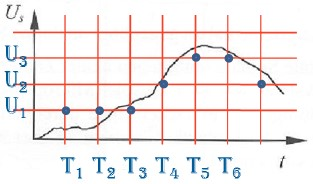
\includegraphics[width=0.9\textwidth]{pics/von_analog_zu_digital.jpg}
	\end{minipage}
	\begin{minipage}[c]{13 cm}
		\begin{minipage}[c]{4 cm}
			Abtasttheorem:
			\newline\newline\newline
			Amplitudenaufl�sung:
			\newline\newline\newline\newline\newline\newline
			Quantisierungsfehler:
			\newline\newline
			dynamischer Bereich AD-Wandler:
		\end{minipage}
		\begin{minipage}[c]{9 cm}
			Nyquist-Shannon besagt, dass ein Signal mit $f_{max}$ mit mindestens einer Frequenz von $2*f_{max}$ abgetastet werden muss, um das Ursprungssignal wieder herzustellen.\\
			Die Anzahl abz�hlbarer Amplitudenwerte (Quantisierungsstufen) bestimmt die Aufl�sung eines AD-Wandlers. Diese wird in der Regel in Bits angegeben. Je kleiner der Bereich aufgeteilt ist, desto kleiner ist der Abstand $\Delta A$ zwischen zwei benachbarten Amplitudenwerten.\\
			Anz. Quantisierungsstufen: $n_{q} = \frac{V_{max} - V{min}}{\Delta A} =$ n \\
			Bei linearer Quantisierung ist der Quantisierungsfehler (Quantisierungsrauschen) max. $\frac{\Delta A}{2}$\\
			\newline
			$DR_{ADC} = U_{max} / U_{min}$\\
			Faustformel: $DR_{ADC}[dB] = 6 * \# Bit$\\
		\end{minipage}
	\end{minipage}

\section{Bin"are Multiplikation}
	\begin{multicols}{2}
		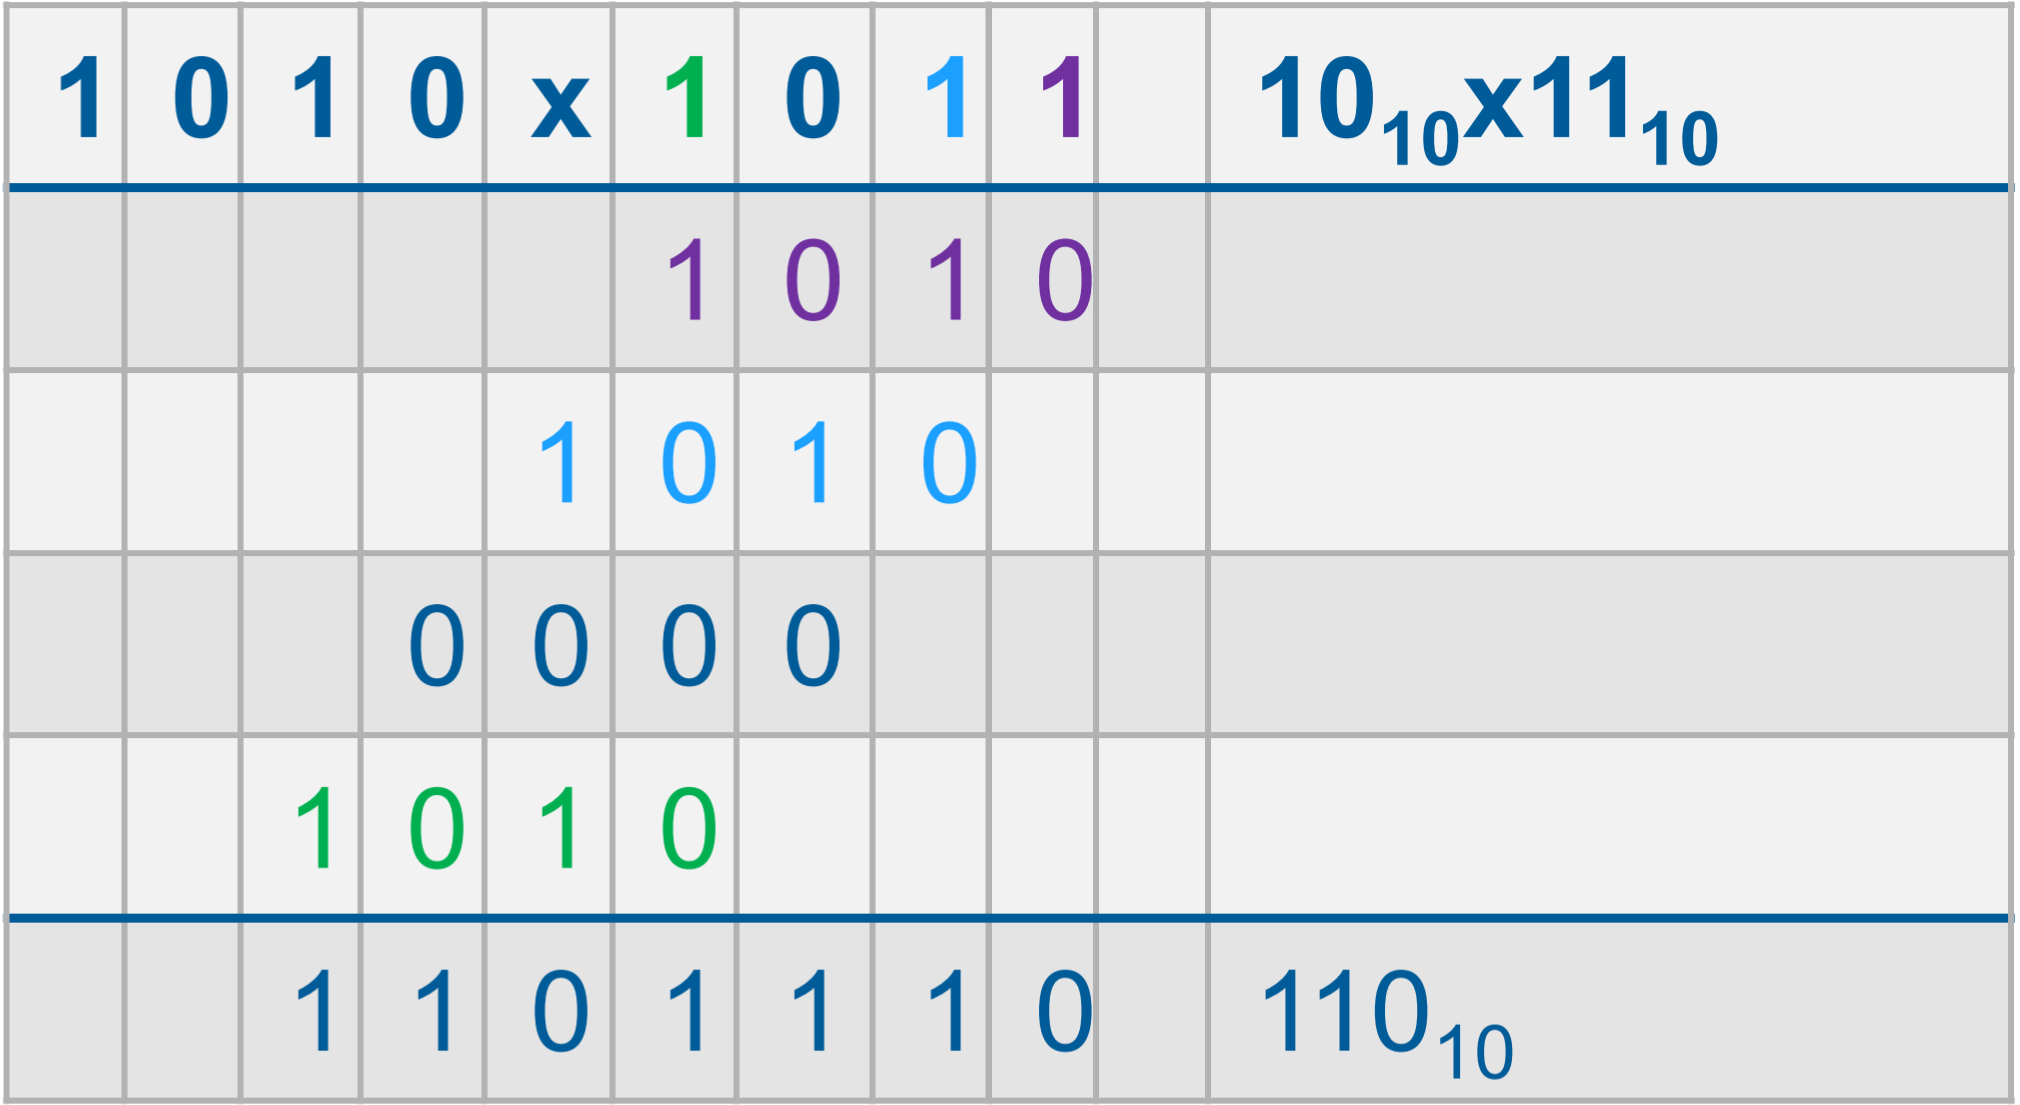
\includegraphics[width=0.7\columnwidth]{pics/multiplikation}
		\columnbreak
		
		Multiplikation von zwei n-Bit W�rtern\\
		Gr�sstes zu erwartendes Ergebnis:\\
		\ \newline
		$E=(2^n-1)*(2^n-1)=2^{2n}-2^{n+1}+1\leq2^{2n}-1$\\
		\ \newline\newline
		Ergebnis kann also max. 2n Bits lang sein!
	\end{multicols}

\section{CMOS Beschaltung}
	\subsection{Beispiel: Inverter}
		\begin{multicols}{2}
			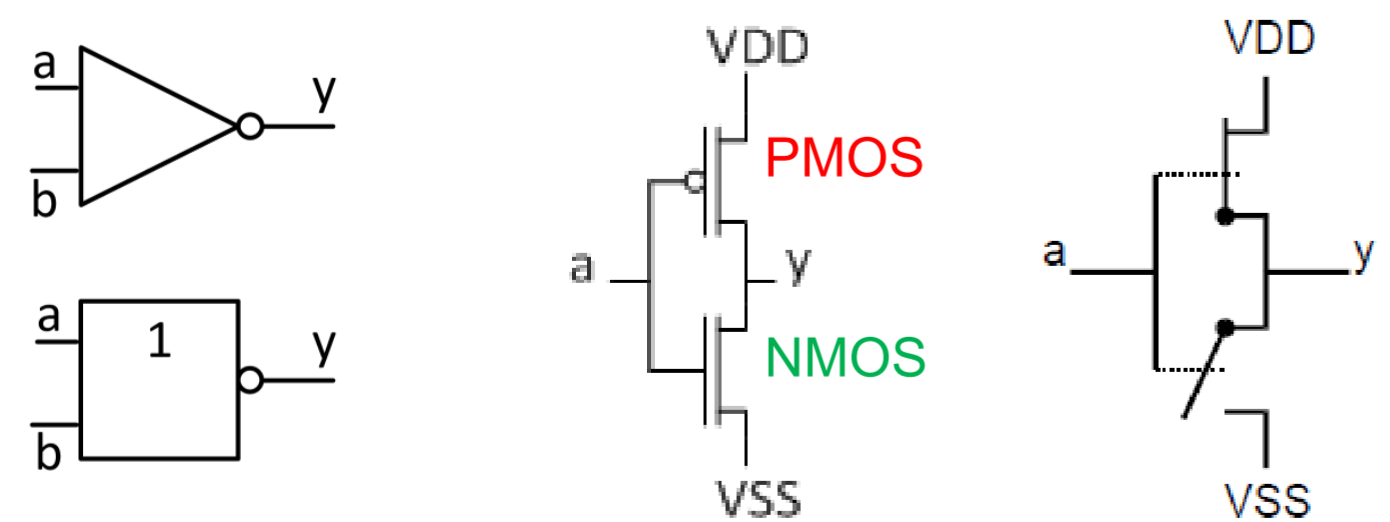
\includegraphics[width=0.5\textwidth]{pics/cmos_transistorenL.png}
			\columnbreak
			
			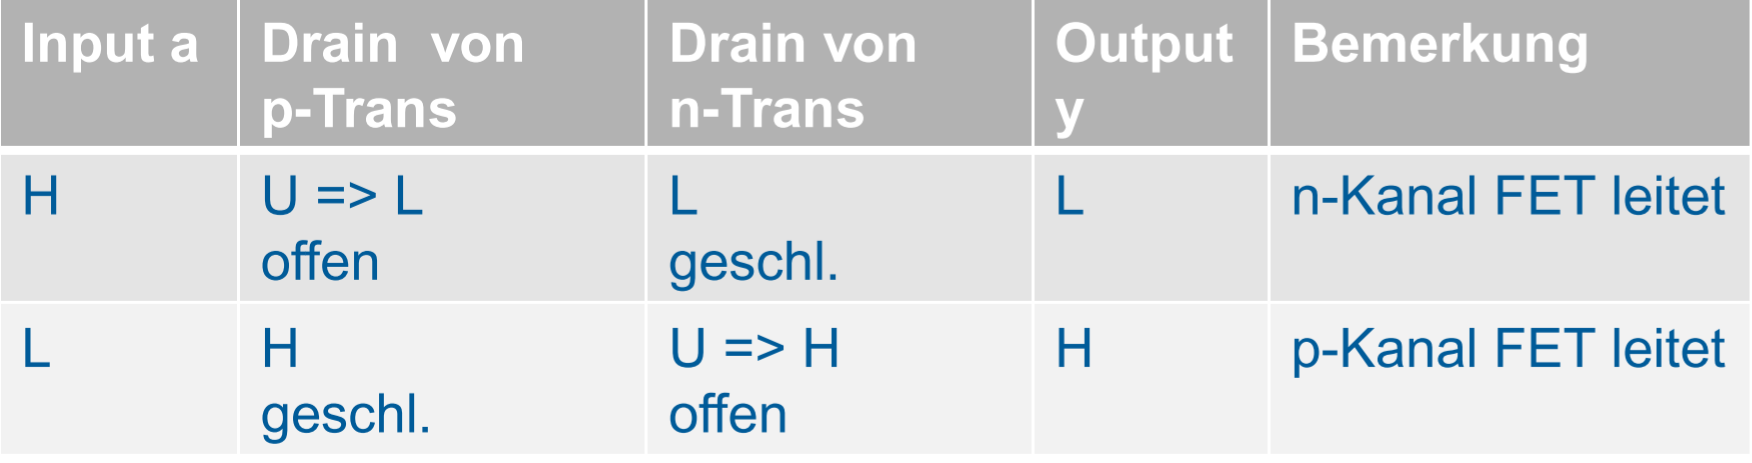
\includegraphics[width=0.5\textwidth]{pics/cmos_transistorenR.png}\newline
			PMOS leitet bei Low-Pegel\\
			NMOS leitet bei High-Pegel\\
			\columnbreak
		\end{multicols}
	
\section{RAM}
	\begin{multicols}{2}
		\subsection{SRAM}
		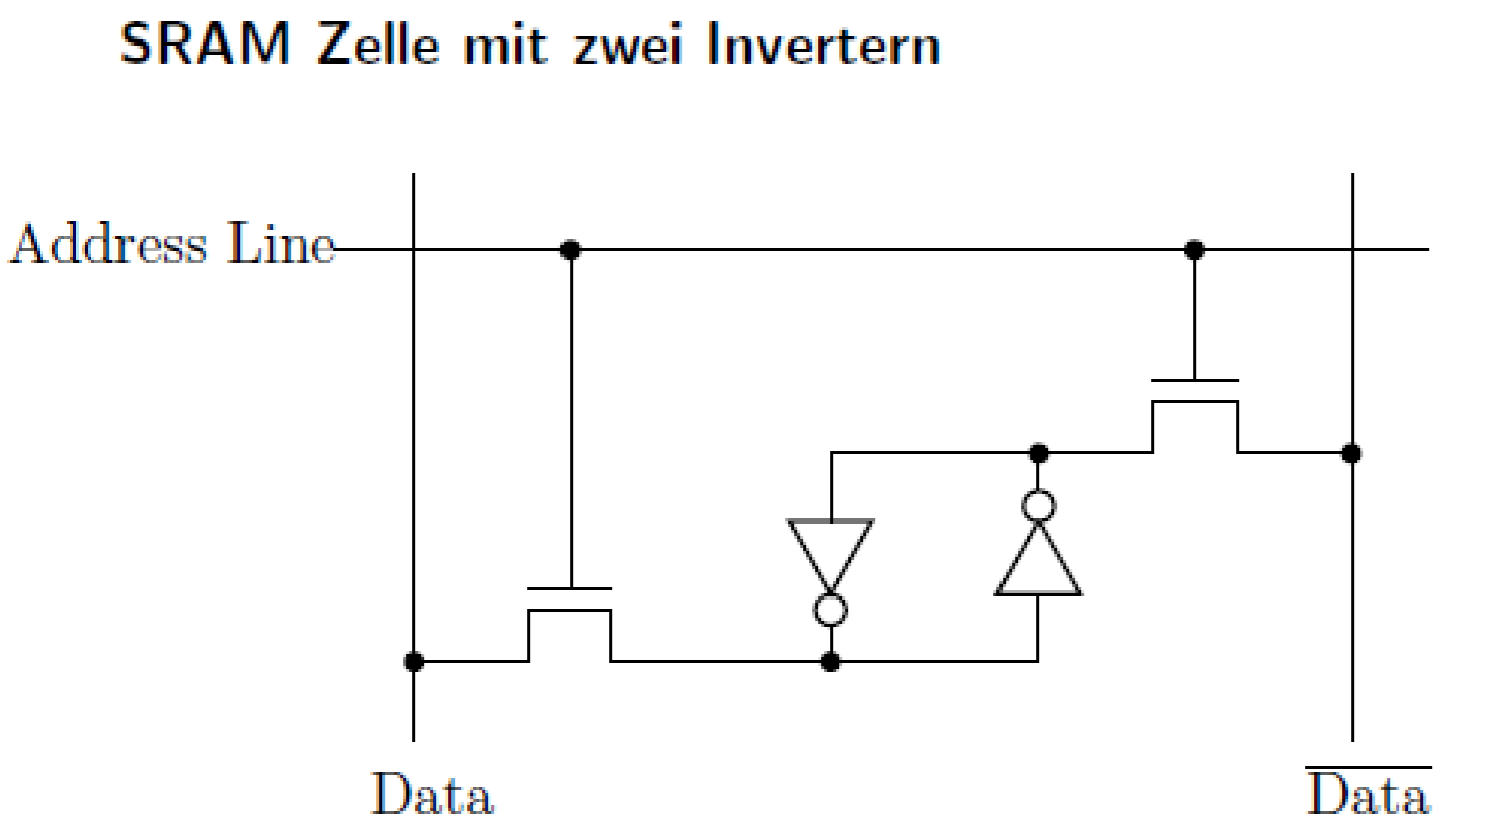
\includegraphics[width=0.5\columnwidth]{pics/sram.png}\newline\newline
		Vorteil: Zustand bleibt, solange Strom vorhanden
			
		\subsection{DRAM}
		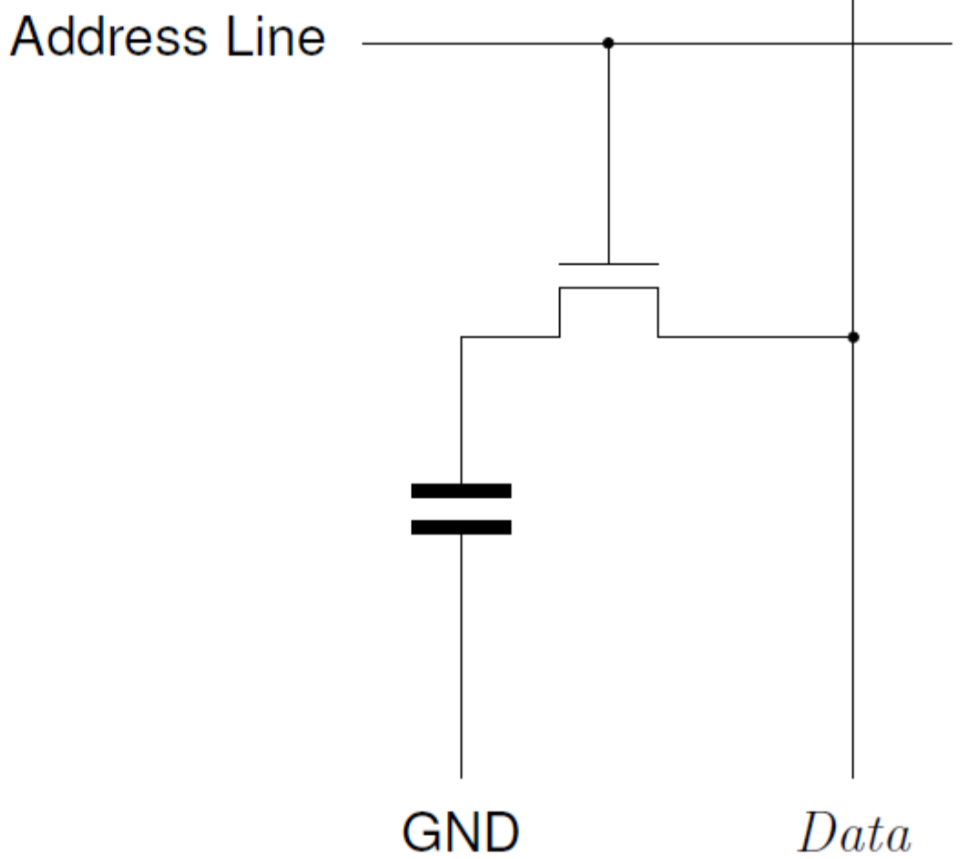
\includegraphics[width=0.3\columnwidth]{pics/dram.png}\newline
		Vorteil: Grosse Dichte einzelner Zellen\\
		Nachteile: \\-Leckstrom Kapazit"at\\
				   -Refresh\\
				   -Steuerlogik\\

		
	\end{multicols}
			

		
	
